\subsubsection{Architektur der Generatoren}
Die Architektur der Generatoren in CycleGAN spielt eine entscheidende Rolle bei der erfolgreichen Durchführung von Bildübersetzungen zwischen verschiedenen Domänen. Typischerweise basieren die Generatoren auf dem ResNet-Ansatz, der für seine Fähigkeit bekannt ist, tiefe neuronale Netze zu trainieren\cite{He.2015}.
\\
\footnote[1]{https://towardsdatascience.com/cyclegan-learning-to-translate-images-without-paired-training-data-5b4e93862c8d}

\begin{figure}[ht]
	\centering
	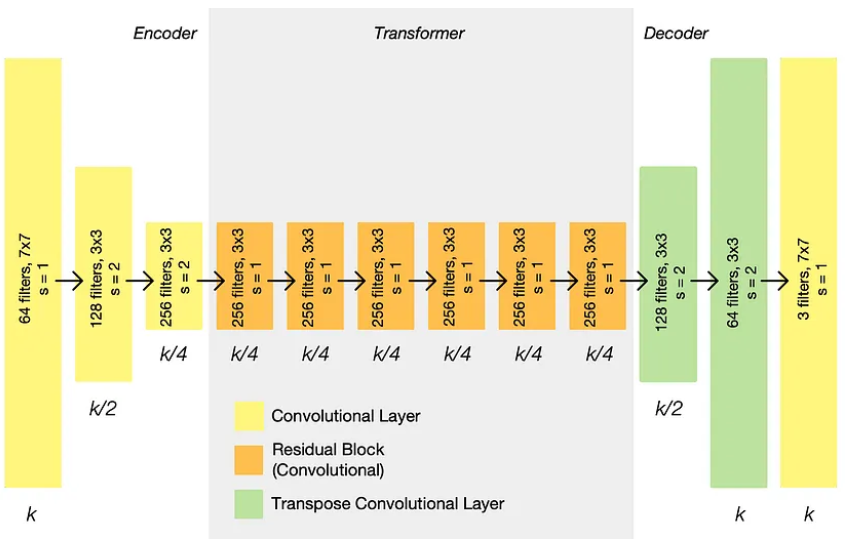
\includegraphics[width=0.8\linewidth]{./images/cycleGanGeneratorArchitecture.png}
	\caption{CycleGAN Generator Achitektur. Instanznormalisierung und ReLU Aktivierung erfolgt nach jeder Schicht
	\protect\footnotemark[1]}
	\label{fig:cycleGanGeneratorArchitecture}
\end{figure}

Im Rahmen der Architektur von Zhu et al. manifestiert sich der Generator im CycleGAN in drei zentralen Abschnitten, wie graphisch in Abbildung \ref{fig:cycleGanGeneratorArchitecture} illustriert. Der Encoder besteht aus drei Convolutional-Schichten, welche unmittelbar auf das Eingabebild einwirken und dabei die Repräsentationsgröße reduzieren sowie die Kanalanzahl erhöhen. Das resultierende Bild unterzieht sich einem Transformer, zusammengesetzt aus mehreren Residualblöcken. Die aus dieser Transformation hervorgehende Repräsentation durchläuft den Decoder, welcher aus zwei Transpose Convolutional-Schichten besteht und somit das Bild erneut vergrößert. Die finale RGB-Ausgabe wird durch eine Ausgabeschicht generiert. Jede dieser Schichten ist mit Instanznormalisierung und ReLU-Aktivierung versehen, was sowohl die Trainingsstabilität fördert, als auch die Qualität der generierten Bilder optimiert\cite{Ulyanov.2016, 10.5555/3104322.3104425}. 
\\
\newline
Die ResNet-Methode, von Kaiming He et al. im Jahr 2015 eingeführt, bietet eine Lösung für das Degradationsproblem. Dieses Phänomen tritt auf, wenn tiefe neuronale Netze bei Zugabe zusätzlicher Schichten schlechtere Leistungen erbringen als flachere Netze, da die Rückwärtspropagierung von Fehlern in tieferen Netzwerken erschwert wird. Die Integration von Residualblöcken ermöglicht die Überwindung dieses Problems durch die Hinzufügung einer Identitätsabbildung. Das Netzwerk lernt diese Abbildung, indem es das Residuum auf Null setzt. Residualblöcke dienen dazu, Änderungen und Fehler zu erlernen, die notwendig sind, um von der Eingabe zur gewünschten Ausgabe zu gelangen. Dies wird durch Shortcut-Verbindungen realisiert, die eine oder mehrere Ebenen überspringen und am Ende einer gestapelten Schicht hinzugefügt werden. Solche Verbindungen fügen keine zusätzlichen Parameter oder Rechenleistung hinzu, und das gesamte Netzwerk kann weiterhin mittels stochastischem Gradientenabstieg (SDG) trainiert werden\cite{He.2015}.
Der Generator des CycleGANs besteht aus sechs Residualblöcken, wobei jeder Block aus zwei Convolutional-Schichten besteht, gefolgt von Instanznormalisierung und ReLU-Aktivierung, wie in Abbildung \ref{fig:residualBlock} dargestellt.

\begin{figure}[ht]
	\centering
	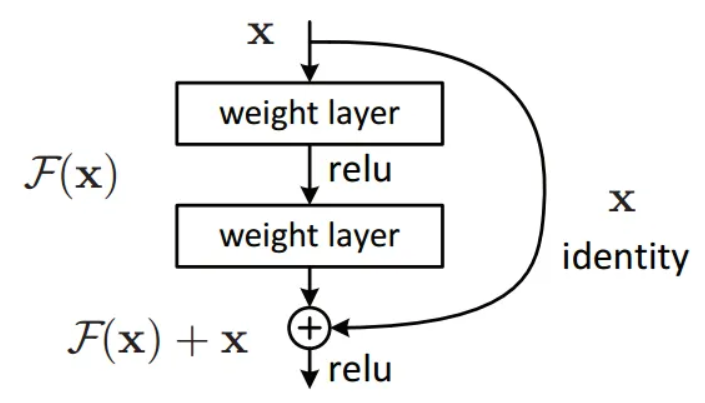
\includegraphics[width=0.5\linewidth]{./images/residualBlock.png}
	\caption{Aufbau Residualblock}
	\label{fig:residualBlock}
\end{figure}

\subsubsection{Architektur der Diskriminatoren}
// TODO: VERGLEICH MIT PIX2PIX
Wie bei Pix2Pix ist die übliche Architektur für Diskriminatoren in CycleGAN PatchGAN, wobei das Bild in kleine Patches aufgeteilt wird und jeder Patch separat klassifiziert wird. Diese Methode ermöglicht eine feine Unterscheidung zwischen echten und generierten Bildern auf lokaler Ebene \cite{Zhu.2017}.

Die Diskriminatoren bestehen in der Regel aus Convolutional Layer, gefolgt von Normalization Layer und Activation Function. In einigen Implementierungen von CycleGAN wird die instanzielle Normalisierung der üblichen Batch-Normalisierung vorgezogen \cite{}.
\\
Die instanzielle Normalisierung ist eine Variante der Normalisierung, die auf Instanzebene durchgeführt wird. Im Gegensatz zur Batch-Normalisierung, bei der die Normalisierung über die gesamte Batch-Dimension durchgeführt wird, wird bei der Instanz-Normalisierung jede Instanz bzw. jedes Bild einzeln betrachtet. Dies kann besonders vorteilhaft sein, wenn die statistischen Eigenschaften der einzelnen Instanzen variieren.

Die Verwendung der Instanznormalisierung in den Diskriminatoren von CycleGAN kann helfen, eine stabilere und konsistentere Konvergenz während des Trainings zu erreichen.

\subsubsection{Training}
Das Training von CycleGAN erfolgt nach einem kompetitiven Verfahren. Die Generatoren $G:X\rightarrow Y$ und $F:Y\rightarrow X$ konkurrieren mit den entsprechenden Diskriminatoren $D_X$ und $D_Y$. $D_X$ versucht, die von $F$ erzeugten Bilder von den echten Bildern aus $X$ zu unterscheiden, während $D_Y$ versucht, die von $G$ erzeugten Bilder von den echten Bildern aus der Domäne $Y$ zu unterscheiden. Die adversen Verluste sind so optimiert, dass die erzeugten Bilder für die Diskriminatoren kaum von den echten Bildern zu unterscheiden sind. \cite{Zhu.2017}.

\subsubsection{Cycle - Konsistenz}
CycleGAN führt zusätzlich eine Cycle-Konsistenz ein. Diese stellt sicher, dass die Übersetzungen zwischen den Domänen sowohl vorwärts ($X$ nach $Y$) als auch rückwärts ($Y$ nach $X$) konsistent sind.
\\
Die Kernidee besteht darin, dass nach der Übersetzung von $X$ nach $Y$ und zurück nach $X$ das resultierende Bild dem ursprünglichen $X$ entsprechen sollte. Um dies zu erreichen, wird die Differenz zwischen dem Originalbild $x$ und dem zyklisch übersetzten Bild $F(G(x))$ mit Hilfe der L1-Verlust minimiert. 
\\
Durch die Einführung dieser zyklischen Konsistenz wird das Problem des Modekollapses gelöst. Die weitere Verlustfunktion stellt sicher, dass die generierten Bilder mehr Strukturen enthalten und somit konsistentere Übersetzungen zwischen den Domänen liefern \cite{Zhu.2017}.

\begin{figure}[ht]
	\centering
	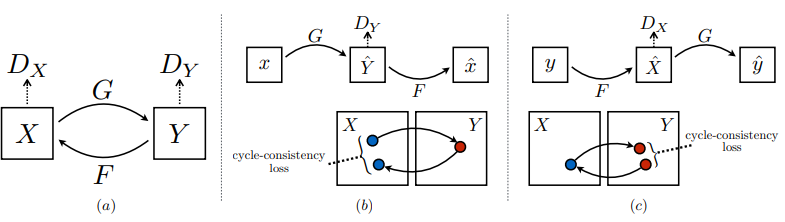
\includegraphics[width=1\linewidth]{./images/cycle_consistency_loss.png}
	\caption{(a) Modell des CycleGANs, bestehend aus zwei Generatoren $F:Y\rightarrow X$ und $G:X \rightarrow Y$ und zugehörige adversarielle Diskriminatoren $D_X$ und $D_Y$,
     (b) Cycle-Konsistenz $F(G(x))\approx x$,
     (c) Cycle-Konsistenz $G(F(y))\approx y$\cite{Zhu.2017}}
	\label{fig:cycleConsistency}
\end{figure}

\subsubsection{Identity - Loss}
Zusätzlich zu den adversariellen und zyklischen Verlusten kann ein Identitätsverlust in die Gesamtverlustfunktion integriert werden, um sicherzustellen, dass die Farbkomposition des Eingabebildes beibehalten wird, während es ins Ausgabebild übersetzt wird. Insbesondere bei der Erstellung von Fotografien aus Gemälden hat sich diese Methode bewährt.  
Wenn der Generator $G$ ein Bild aus dem Bereich $Y$ erhält, darf es sich aufgrund seiner bereits vorhandenen Zugehörigkeit zu diesem Bereich nicht mehr verändern. 
Der Verlust wird dabei mittels des L1-Verlust ermittelt, bei dem die Differenz zwischen den Pixeln des generierten Bildes $G(y)$ und dem Referenzbild $y\in Y$ erfasst wird. Das gleiche Verfahren wird für den anderen Generator $F$ angewendet \cite{Zhu.2017}

\begin{figure}[h]
	\centering
	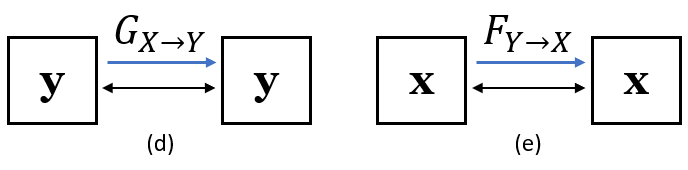
\includegraphics[width=0.7\linewidth]{./images/identity_loss.png}
	\caption{Identity-Mapping für (d) Generator $G$ und (e) Generator $F$}
	\label{fig:IdentityMapping}
\end{figure}


\subsection{Anwendungen von CycleGAN}
CycleGAN hat sich als äußerst vielseitiges Modell erwiesen und wird in verschiedenen Anwendungsbereichen eingesetzt. Die Fähigkeit, Bildübersetzungen zwischen unpaaren Domänen durchzuführen, hat zu zahlreichen innovativen Anwendungen geführt.
\\
Eine der prominentesten Anwendungen von CycleGAN ist die Bild-zu-Bild-\\Übersetzung. Dies beinhaltet die Transformation von Bildern zwischen verschiedenen Stilen, Szenarien oder Kunstwerken. Beispielsweise kann CycleGAN verwendet werden, um Fotos in den Stil berühmter Kunstwerke zu transformieren, was einen einzigartigen und kreativen Ansatz für die Bildbearbeitung bietet.
Ein weiteres Anwendungsgebiet von CycleGAN ist die Stilübertragung. Hier können Stile von einem Bild auf ein anderes übertragen werden, ohne dass gepaarte Trainingsdaten benötigt werden. So ist es möglich, den Stil eines Gemäldes auf ein fotografisches Bild zu übertragen oder umgekehrt. CycleGAN kann auch für die Übersetzung zwischen verschiedenen Farbbereichen verwendet werden. Zum Beispiel kann es verwendet werden, um Schwarz-Weiß-Bilder in Farbversionen zu übersetzen oder den Farbton von Bildern anzupassen, ohne dass gepaarte Trainingsdaten benötigt werden.
